\documentclass[11pt]{article}
\usepackage[landscape]{geometry}
\usepackage{calc}
\usepackage{tikz}
\usetikzlibrary{arrows,decorations.markings}
%\tikzstyle{vertex}=[circle, draw, inner sep=0pt, minimum size=18pt]
\tikzstyle{vertex}=[circle, fill=black, draw, inner sep=0pt, minimum size=5pt]

\newcommand{\vertex}{\node[vertex]}
\newcounter{Angle}
\pagestyle{empty}
\begin{document}
{\large\bf
\[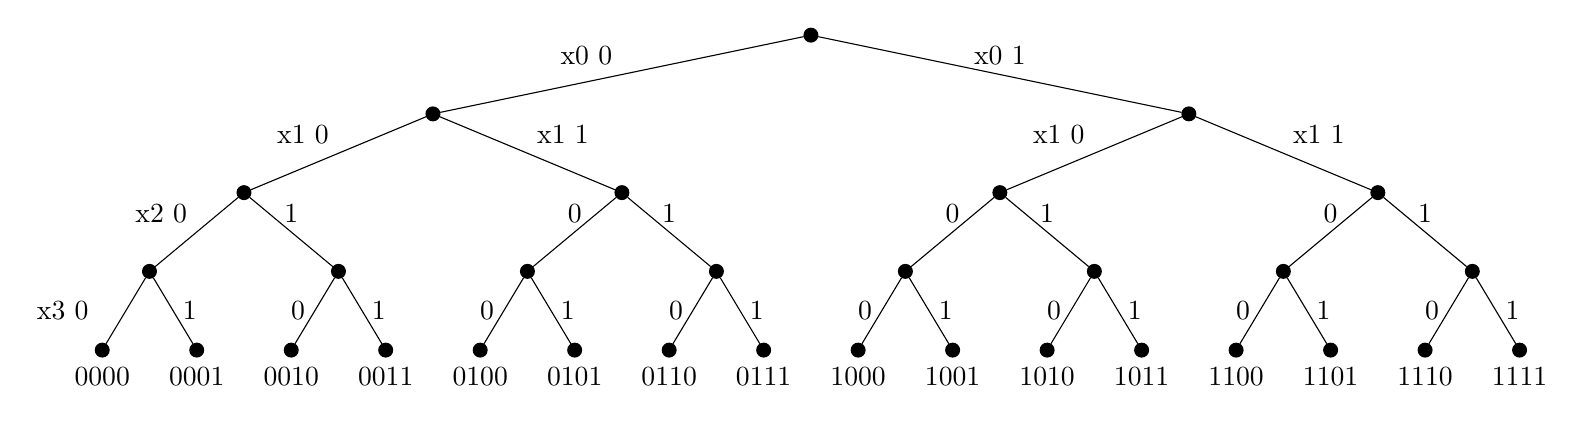
\begin{tikzpicture}[x=.6cm, y=1cm, every edge/.style={ draw } ]
\vertex (0) at (0,0) [label=below:{0000}]{};
\vertex (1) at (1,1) {};
\vertex (2) at (2,0) [label=below:{0001}]{};
\vertex (3) at (3,2) {};
\vertex (4) at (4,0) [label=below:{0010}]{};
\vertex (5) at (5,1) {};
\vertex (6) at (6,0) [label=below:{0011}]{};
\vertex (7) at (7,3) {};
\vertex (8) at (8,0) [label=below:{0100}]{};
\vertex (9) at (9,1) {};
\vertex (10) at (10,0)  [label=below:{0101}]{};
\vertex (11) at (11,2) {};
\vertex (12) at (12,0)  [label=below:{0110}]{};
\vertex (13) at (13,1) {};
\vertex (14) at (14,0) [label=below:{0111}]{};
\vertex (15) at (15,4) {};
\vertex (16) at (16,0)  [label=below:{1000}]{};
\vertex (17) at (17,1) {};
\vertex (18) at (18,0) [label=below:{1001}]{};
\vertex (19) at (19,2) {};
\vertex (20) at (20,0) [label=below:{1010}]{};
\vertex (21) at (21,1) {};
\vertex (22) at (22,0)  [label=below:{1011}]{};
\vertex (23) at (23,3) {};
\vertex (24) at (24,0) [label=below:{1100}]{};
\vertex (25) at (25,1) {};
\vertex (26) at (26,0) [label=below:{1101}]{};
\vertex (27) at (27,2) {};
\vertex (28) at (28,0) [label=below:{1110}]{};
\vertex (29) at (29,1) {};
\vertex (30) at (30,0) [label=below:{1111}]{};
\path 
(1) edge node [left] {x3 0 \ \ \ } (0) edge node [right] {1} (2) edge node [above left] {x2 0} (3)
(5) edge node [left] {0} (4) edge node [right] {1} (6) edge node [above] {1} (3)
(9) edge node [left] {0} (8) edge node [right] {1} (10) edge node [above] {0} (11)
(13) edge node [left] {0} (12) edge node [right] {1} (14) edge node [above] {1} (11)
(17) edge node [left] {0} (16) edge node [right] {1} (18) edge node [above] {0} (19)
(21) edge node [left] {0} (20) edge node [right] {1} (22) edge node [above] {1} (19)
(25) edge node [left] {0} (24) edge node [right] {1} (26) edge node [above] {0} (27)
(29) edge node [left] {0} (28) edge node [right] {1} (30) edge node [above] {1} (27)
(7) edge node [above left] {x1 0} (3) edge node [above right] {x1 1} (11) edge node [above left] {x0 0} (15)
(23) edge node [above left] {x1 0} (19) edge node [above right] {x1 1} (27) edge node [above] {x0 1} (15)
;
\end{tikzpicture}\]
\[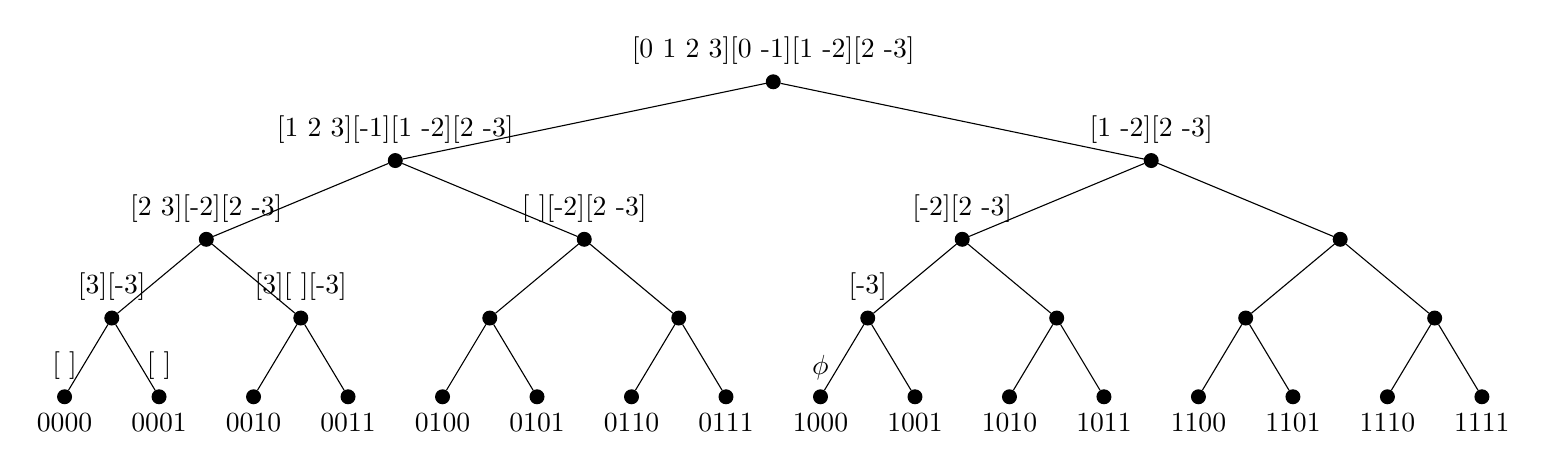
\begin{tikzpicture}[x=.6cm, y=1cm, every edge/.style={ draw } ]
\vertex (0) at (0,0) [label=above:{[ ]}][label=below:{0000}]{};
\vertex (1) at (1,1) [label=above:{[3][-3]}]{};
\vertex (2) at (2,0) [label=above:{[ ]}][label=below:{0001}]{};
\vertex (3) at (3,2) [label=above:{[2 3][-2][2 -3]}]{};
\vertex (4) at (4,0) [label=below:{0010}]{};
\vertex (5) at (5,1) [label=above:{[3][ ][-3]}]{};
\vertex (6) at (6,0) [label=below:{0011}]{};
\vertex (7) at (7,3) [label=above:{[1 2 3][-1][1 -2][2 -3]}]{};
\vertex (8) at (8,0) [label=below:{0100}]{};
\vertex (9) at (9,1) {};
\vertex (10) at (10,0)  [label=below:{0101}]{};
\vertex (11) at (11,2) [label=above:{[ ][-2][2 -3]}]{};
\vertex (12) at (12,0)  [label=below:{0110}]{};
\vertex (13) at (13,1) {};
\vertex (14) at (14,0) [label=below:{0111}]{};
\vertex (15) at (15,4) [label=above:{[0 1 2 3][0 -1][1 -2][2 -3]}]{};
\vertex (16) at (16,0) [label=above:{$\phi$}][label=below:{1000}]{};
\vertex (17) at (17,1) [label=above:{[-3]}]{};
\vertex (18) at (18,0) [label=below:{1001}]{};
\vertex (19) at (19,2) [label=above:{[-2][2 -3]}]{};
\vertex (20) at (20,0) [label=below:{1010}]{};
\vertex (21) at (21,1) {};
\vertex (22) at (22,0)  [label=below:{1011}]{};
\vertex (23) at (23,3) [label=above:{[1 -2][2 -3]}]{};
\vertex (24) at (24,0) [label=below:{1100}]{};
\vertex (25) at (25,1) {};
\vertex (26) at (26,0) [label=below:{1101}]{};
\vertex (27) at (27,2) {};
\vertex (28) at (28,0) [label=below:{1110}]{};
\vertex (29) at (29,1) {};
\vertex (30) at (30,0) [label=below:{1111}]{};
\path 
(1) edge (0) edge (2) edge (3)
(5) edge (4) edge (6) edge (3)
(9) edge (8) edge (10) edge (11)
(13) edge (12) edge (14) edge (11)
(17) edge (16) edge (18) edge (19)
(21) edge (20) edge (22) edge (19)
(25) edge (24) edge (26) edge (27)
(29) edge (28) edge (30) edge (27)
(7) edge (3) edge (11) edge (15)
(23) edge (19) edge (27) edge (15)
;
\end{tikzpicture}\]
}
\end{document}
